% Nejprve uvedeme tridu dokumentu s volbami
\documentclass[czech,bachelor,dept460,male,cpp,cpdeclaration]{diploma}
% Dalsi doplnujici baliky maker
\usepackage[autostyle=true,czech=quotes]{csquotes} % korektni sazba uvozovek, podpora pro balik biblatex
\usepackage[backend=biber, style=iso-numeric, alldates=iso]{biblatex} % bibliografie
\usepackage{dcolumn} % sloupce tabulky s ciselnymi hodnotami
\usepackage{subfig} % makra pro "podobrazky" a "podtabulky"

% Zadame pozadovane vstupy pro generovani titulnich stran.
\ThesisAuthor{Filip Peterek}

\CzechThesisTitle{Vývoj samoříditelné platformy}

\EnglishThesisTitle{Self-driving Platform Development}

\SubmissionDate{30. dubna 2021}

% Pokud nechceme nikomu dekovat makro zapoznamkujeme.
\Thanks{
	Chtěl bych poděkovat vedoucímu mé práce, Ing. Janu Gaurovi, nejen za pomoc s tvorbou práce a návrhem softwaru,
	ale především za možnost se projevit a pracovat na skutečném a zajímavém projektu. Dále chci poděkovat svým
	kolegům z práce, kteří mě naučili spoustu věcí, na které v akademickém prostředí není čas nebo příležitost.
}

% Zadame cestu a jmeno souboru ci nekolika souboru s digitalizovanou podobou zadani prace.
% Pokud toto makro zapoznamkujeme sazi se stranka s upozornenim.
\ThesisAssignmentImagePath{Figures/Assignment}

% Zadame soubor s digitalizovanou podobou prohlaseni autora zaverecne prace.
% Pokud toto makro zapoznamkujeme sazi se cisty text prohlaseni.
\AuthorDeclarationImageFile{Figures/AuthorDeclaration.jpg}


% Zadame soubor s digitalizovanou podobou souhlasu spolupracujici prav. nebo fyz. osoby.
% Pokud toto makro zapoznamkujeme sazi se cisty text souhlasu.
\CooperatingPersonsDeclarationImageFile{Figures/CoopPersonDeclaration.jpg}

\CzechAbstract{
	Tato práce se zabývá vývojem software pro samořiditelnou platformu vznikající na VŠB-TUO. Po dokončení by software
	měl být schopen na základě vstupů ze softwaru pro analýzu obrazu, GPS, Lidaru a řídící jednotky vozidla bezpečně
	navigovat vozidlo univerzitním kampusem.

	Řídící software je rozdělen do dvou komponent. První komponenta zajišťuje komunikaci s řídící jednotkou vozidla
	pomocí sběrnice CAN, na starosti má ovládání rychlosti vozidla a natáčení kol. Druhá komponenta má na starosti
	plánování cesty na základě výše vyjmenovaných vstupů. První komponentě poté zadá pouze požadovanou rychlost vozidla
	a natáčení kol, samotné posílání CAN zpráv však nemusí řešit. Komponenty mezi sebou komunikují pomocí protokolu TCP.
	K testování ovládacího software lze využít simulátor, který dokáže nasimulovat chování první komponenty. Pro řízení
	vozidla jsou v hojné míře využívány PID regulátory.

	V době odevzdání této práce ještě není software plně dokončený, jelikož se jedná o výzkumný projekt, který svým
	rozsahem přesahuje bakalářskou práci, a vývoj platformy bude dále pokračovat.
}

\CzechKeywords{
	plánování cesty, client-server komunikace, sběrnice CAN, PID regulátor
}

\EnglishAbstract{
	This thesis is focused on the development of software for a self-driving platform, which is being developed by
	the Technical University of Ostrava. Upon completion, the software should be capable of safely navigating an
	autonomous vehicle through the university campus, taking inputs from image analysis software, GPS, Lidar, and the
	vehicle's own controller unit.

	The software is split into two components. The first component handles communication with the vehicle's controller
	unit via a CAN bus. The second component then does all the path planning, taking into account the aforementioned
	inputs. The second component then asks the first component to maintain a certain speed or steer the vehicles,
	however, it doesn't have to handle CAN messages, including driving inputs or control checksums, by itself. The TCP
	protocol is used for communication between the components. The path planning software can be tested using
	a simulator, capable of mocking the CAN handling software, along with the entire vehicle. The simulator honors
	the TCP API, however, the vehicle physics are simplified. PID controllers are used in multiple parts of the
	software.

	At the time of publishing this paper, the software is still unfinished, as the self-driving platform is an academic
	research project, which outspans this bachelor's thesis in scope, and development of the platform will continue.
}

\EnglishKeywords{
	path planning, client-server communication, CAN bus, PID controller
}

\AddAcronym{CAN}{Controller Area Network}
\AddAcronym{PID}{Proporcionální-integrační-derivační}
\AddAcronym{TCP}{Transmission Control Protocol}
\AddAcronym{GPS}{Global Positioning System}
\AddAcronym{API}{Application Programming Interface}
\AddAcronym{XML}{Extensible Markup Language}
\AddAcronym{JSON}{JavaScript Object Notation}
\AddAcronym{TX}{Transmitter}
\AddAcronym{RX}{Receiver}
\AddAcronym{RPC}{Remote Procedure Call}

\addbibresource{biblatex-examples.bib}
\addbibresource{coffee.bib}

% Novy druh tabulkoveho sloupce, ve kterem jsou cisla zarovnana podle desetinne carky
\newcolumntype{d}[1]{D{,}{,}{#1}}


% Zacatek dokumentu
\begin{document}

% Nechame vysazet titulni strany.
\MakeTitlePages

% A nasleduje text zaverecne prace.
\section{Úvod}
\label{sec:Introduction}
Tato práce je součást většího výzkumného projektu. Cílem projektu je vývoj autonomního eletrifikovaného vozidla, 
od fyzického návrhu a zkonstruování vozidla, až po vývoj softwaru. Hotové vozidlo má být schopno plně autonomního pohybu
po univerzitním kampusu, kde má sloužit k rozvozu materiálu napříč budovami. Při tvorbě samořiditelné platformy je nutné
klást vysoký důraz na bezpečnost provozu, výsledek projektu při reálném využití nesmí ohrozit zdraví ani majetek 
univerzity nebo jejích návštěvníků. 

Samotná práce se zabývá vývojem řídícího softwaru vozidla. Software bude sloužit k navigaci vozidla areálem univerzity, 
plánování cesty, a zajištění bezpečnosti provozu. Pro tento účel řídící kód využívá vstupy z GPS, kamer, Lidaru, 
a ovládací jednotky vozidla. Analýza obrazu a dat naměřených Lidarem není předmětem této práce, výsledek této analýzy 
je získáván z API komponenty určené právě k tomuto účelu, taktéž vyvíjené jako součást projektu.

Software, který je vyvíjen jako součást této práce, je tvořen v Pythonu, a je rozdělen do více komponent. Kromě řídícího
softwaru byl vyvinut také jednoduchý simulátor, umožňující testování řízení. Dále řídící software obsahuje funkční 
vizualizér, pomocí kterého je možné sledovat pohyb vozidla. Při tvorbě řídících komponent byla využita řada open source
knihoven a veřejných zdrojů, včetně map OpenStreetMap nebo Mapy.cz. Zdrojový kód, který je součástí této práci, je 
rovněž otevřený a veřejně dostupný na Githubu.

\section{Architektura řídícího softwaru}
Jak již bylo zmíněno, řídící software je rozdělen do dvou komponent, komunikujících mezi sebou pomocí protokolu TCP na bázi 
architektury klient-server. Jako server slouží program zajišťující přenos dat na rozhraní CAN. Server takto abstrahuje 
nízkoúrovňové a bezpečnostní záležitosti, mezi které patří výpočet kontrolních součtů, zasílání CAN zpráv, TX/RX synchronizace, 
žádání o možnost ovládat vozidlo, regulace rychlosti pomocí PI regulátoru, nebo také zpracování výstupu z GPS modulu. Klient tak
může implementovat pouze samotné plánování cesty, v dotazech na server stačí žádat pouze o dodržování rychlosti, úhlu natočení 
kol, případně aplikace nouzové brzdy. Server samozřejmě dokáže poskytovat zpětnou vazbu, tedy informace o aktuální rychlosti,
pozici, natočení kol, nebo zdraví systému (tzv. \emph{healthcheck}). Server je většinou spouštěn na Raspberry Pi, ačkoliv může
být spouštěn na libovolné jednotce připojené k rozhraní CAN samořiditelné platformy, za předpokladu, že je na dané jednotce
nainstalován interpreter jazyka Python.

Toto dělení nejen zvyšuje úroveň abstrakce, a tím i čitelnost kódu, ale zároveň umožňuje spustit program plánující 
cestu vozidla na vzdáleném stroji. Takto můžeme například program spouštět na výkonnějším stroj a vyhnout se omezením 
Raspberry Pi, virtualizovat ovládací software, nebo implementovat jiný typ klienta, které v současné době existují tři.
Jeden klient se snaží vozidlo řídit na základě vstupů ze senzorů umístěných na vozidle a z komponenty určené pro analýzu obrazu. 
Druhý klient umožňuje řídící pokyny zadávat manuálně do jednoduchého textového prostředí. Třetí klient poté pouze pošle 
předdefinovanou testovací sekvenci. Druhý a třetí klient jsou určeny pouze k ověření funkčnosti komunikace pomocí sběrnice CAN. 
Virtualizace ovládacího softwaru také umožňuje zautomatizovat monitorování ovládání. Ačkoliv k žádným pokusům o automatickou 
orchestraci a monitorování zatím nedošlo, bylo by možné například spouštět řídící software v Kubernetes, nastavit kontinuální 
nasazování pomocí CI/CD pipeline, a logy či metriky kontrolovat strojově pomocí nástrojů jako ELK stack nebo Prometheus.

\section{Server a CAN komunikace}

\subsection{Sběrnice CAN}

Controller Area Network, zkráceně CAN, je standard poskytující určitý základ pro komunikaci na sběrnici. Standard definuje
fyzické požadavky na sběrnici a formát zpráv. Součástí zprávy je osm bytů vyhrazených pro data. Sběrnice CAN je, mimo jiné, hojně
využívána právě v automobilovém průmyslu.

\subsubsection{Vlastní specifikace}
Standard sice přiřazuje každé zprávě osmibytové pole vyhrazené pro data, již však nedefinuje, jaká data mají zprávy obsahovat, 
v jakém formátu mají být data posílána, nebo jak se s nimi má pracovat. Obsah zpráv tak musel být vydefinován vlastní specifikací, 
která prošla hned několika iteracemi, a jejíž finální podoba je výsledkem úzké spolupráce konstruktérů fyzické platformy a tvůrců 
řídícího softwaru. Specifikace byla navrhována tak, aby umožnila dostatečně jemné řízení vozidla, poskytovala řídícímu softwaru
všechna potřebná jízdní data a zahrnovala množství prostředků pro kontrolu integrity zprávy, rychlé zachycení chyb či reportování
problémů. Na chyby nebo problémy je samozřejmě důležité reagovat, v krajních případech až nouzovým zastavením vozidla. Software
pro ovládání platformy byl již několikrát přepisován na základě upravené specifikace, nejaktuálnější verze software však 
implementuje nejnovější verzi specifikace.

\subsection{TCP server a jeho metody}

Za účelem zvýšení abstrakce a zjednoduššení ovládání vozidla, ale také aby bylo umožněno vzdálené ovládání platformy
a zjednodušila se výměna způsobů ovládání, je nízkoúrovňové řízení CAN zprávami abstrahováno a obaleno jednoduchým TCP serverem.
Při vývoji serveru se přirozeně nabídla možnost implementace REST API a využití protokolu HTTP, nebo využití jednoho z rozšířených
RPC prokolů, jako jsou XMLRPC nebo gRPC. Ačkoliv validní, tyto způsob, implementace se jevily jako neefektivní -- rozhraní 
poskytované serverem je velmi jednoduché, plaintextový protokol HTTP nebo variace protokolů RPC tak působily až zbytečně 
komplikovaně. Pro komunikaci byl nakonec použit vlastní binární protokol a jeho implementace přímo nad TCP sockety. 
Výhodou je rychlost a jednoduchost implementace, úspornost a výkonnost řešení v reálném provozu, nebo fakt, že toto řešení 
nevyžaduje žádné externí závislosti nad rámec standardní knihovny jazyka Python. Nevýhody současného řešení by se projevily 
pouze při výrazném nárůstu komplexity poskytovaného rozhraní. Tento scénář by mohl vést k znepřehlednění současného řešení. 
Nutnosti zvyšování komplexity rozhraní ovšem v současné době nic nenasvědčuje. 

Aktuální verze serveru implementuje celkem pět metod. Na vstupu přijímá celkem tři byty. První byte je vyhrazen pro identifikaci 
metody serveru. Následující dva byty dotazu obsahují data. Klient musí vždy poslat minimálně tři byty, na vstupu jsou, nezávisle
na metodě, pokaždé očekávány tři byty. Jestliže klient pošle v dotazu více než dva datové byty, budou nadbytečná data ignorována.

Jako identifikátor metody je využito celé nezáporné číslo. V případě, že první byte zprávy obsahuje identifikátor nepříslušící 
žádné metodě, je dotaz ignorován. Obsah datových bytů je určen danou metodou serveru. Pokud pro danou funkcionalitu není třeba 
předávat serveru žádná data, může být obsah datových bytů libovolný, data budou ignorována. 

\subsubsection{Metoda \emph{drive}}
Metoda \emph{drive} slouží k předání požadované rychlosti vozidla a natočení kol. Obsah první datového bytu je interpretován jako 
rychlost, druhý datový byte reprezentuje natočení předních kol. Oba datové byty jsou interpretovány jako celá znaménková čísla. 

Fyzická změna rychlosti nebo natočení kol samozřejmě nemůže nastat okamžitě, rychlost změny je omezena fyzikálními vlastnostmi 
konstrukce i PI regulátorem, proto nelze vrátit klientu potvrzení o provedené změně. Odpovědí metody je ekvivalentní s metodou 
\emph{healthcheck}. \emph{Healthcheck} v odpovědi slouží jako potvrzení přijetí dotazu a schopnosti dotazu vyhovět. V případě, 
že klient potřebuje potvrzení o dosažení požadované rychlosti nebo úhlu natočení kol, je možné po zavolání metody \emph{drive} 
opakovaně volat metodu \emph{info}.

\subsubsection{Metoda \emph{healthcheck}}
Metoda \emph{healthcheck} slouží k ověření \emph{živosti} systému. \emph{Živost} je binární stav, systém je buď \emph{živý}, nebo
\emph{mrtvý}. Server je považován za \emph{živý}, jestliže je schopen zpracovávat TCP spojení, a zároveň má plnou kontrolu 
nad vozidlem. V opačném případě je server považován za \emph{mrtvý}. Metoda nepřijímá žádný vstup, datové byty jsou ignorovány.

\emph{Healthcheck} ve své odpovědi posílá pouze jeden byte. Pokud je server živý, obsahuje odpověď nenulovou hodnotu. V opačném
případě vrátí server nulu, nebo neodpoví vůbec.

\subsubsection{Metoda \emph{info}}
\emph{Info} metoda TCP serveru se využívá k získání aktuálních jízdních dat vozidla. Na vstupu nepřijímá žádné parametry, všechny
datové byty jsou tedy ignorovány. Na výstupu server vrátí tři byty. První dva byty reprezentují znaménková celá čísla. Obsahem
prvního bytu je aktuální rychlost vozidla. Druhý byte obsahuje úhel natočení kol. Poslední byte poté obsahuje logickou hodnotu
značící stav nouzové brzdy. Jestliže je hodnota třetího bytu nulová, nouzová brzda není aktivována. Nenulová hodnota značí, 
že došlo k aktivaci nouzového brždění, a bude třeba jej deaktivovat, pokud chceme pokračovat v jízdě.

\subsubsection{Metoda \emph{ebrake}}
\emph{Ebrake}, nebo-li \emph{'Emergency Brake'}, česky 'nouzová brzda', slouží k ovládání nouzového brždění. První byte vstupu
je serverem interpretován jako logická hodnota značící požadovaný stav nouzové brzdy. Nenulovou hodnotu server považuje za signál
k aktivaci nouzového brždění. Při přijetí nulové hodnoty na vstupu poté dochází k deaktivaci nouzové brzdy. Druhý byte vstupu 
je ignorován.

Výstup metody \emph{ebrake} je opět ekvivalentní výstupu metody \emph{healthcheck}. Nenulová hodnota na výstupu značí, že server
požadavek přijal a je schopen jej zpracovat. Nula reprezentuje stav, kdy server nemá kontrolu nad vozidlem a není schopen 
nouzovou brzdu aktivovat. Pokud však ke ztrátě kontroly došlo důsledkem chyby, vozidlo začne nouzově brzdit samo.

\subsubsection{Metoda \emph{position}}

\emph{Position} využijeme, chceme-li zjistit geografickou polohu vozidla. Tato metoda, která neakceptuje žádný vstup, ve svém 
17 bytovém výstupu vrací tři hodnoty. 

První byte obsahuje logickou hodnotu značící, zda je geografická poloha věrohodná. Nulový
byte značí polohu nevěrohodnou, nenulový byte věrohodnou. Poloha je považována za nevěrohodnou např. pokud nedojde ke správné
inicializaci vozidla, GPS modul nedokáže zaměřit pozici, apod. 

V následujících osmi bytech je zakódována zeměpisná šířka (latitude), v posledních osmi bytech pak zeměpisná délka (longitude). 
Ačkoliv se jedná o desetinná čísla, pro zjednodušení jsou zakódována jako čísla celá. Skutečná hodnota zeměpisné šířky a délky 
je vynásobena číslem $10^{10}$ a převedena na celé číslo. Výsledné číslo je poté zakódováno kódováním little endian. Klient tedy 
nesmí při zpracování odpovědi opomenout číslo správně dekódovat.

\subsection{Regulace PI regulátorem}

\subsection{Python implementace}

\begin{lstlisting}[label=src:CppListing,caption={Program Hello world v jazyce C++}]
// My first program in C++
// Příšerně žluťoučký kůň úpěl ďábelské ódy
#include <iostream>

int main(int argc, const char * argv[]) {
	std::cout << "Hello World!" << std::endl;
}

\end{lstlisting}

\begin{lstlisting}[language=Python,label=src:PythonListing,caption={Program Hello world v jazyce Python}]
# Python program Hello, World
my_string = "Hello, World!"
print(my_string)
\end{lstlisting}

Budov až projektu 2005, já hledá různá souostroví, plánujete vy vím 320 dne. Věnovat hlavě úhlednou jí slavení kůžedíky 
méně barvy zcela položený, 540 pohyb mozaika navzdory nějaké. Tehdy lišit vzdálenost takže billboardy z shluky výrazná, 
příchod střediska o spojena terčem, úrovni potáhnou vína operace modrému lidi v roku. Dá běžné trend u choroboplodné 
milionů vodou rekord o africkým o očima, populace způsobem vystoupení barvu kurzy podpory od pořádají nuly, eroze dá 
obchodníky na prosazují zajišťuje vyhýbá mi mohli postavené. U připlouváte léta technologií, chyba nejhlubší toto četné 
k stopy. Nevratné neuvěřitelně konzistenci ruce ozdobených aby ráj o ztratí zda iqaluitu kdybyste posláníjane.

\subsection{Důležití sezonní za úspěch}
Včera a začít lingvistiku lyžaři mého dubnu, i u annan lodní američtí ji druhy párová, vědců potřebám chránit v vysocí 
mi prostředí zaledněné u hledá s přibližně zpráv mocná hospodářské pohroma. Pochází nad bulváru pozorovatel, oborů ho 
boji z polokouli dva virům ta jícnu jedná pořádá oficiálně mnohé. Vy nezbytné kaple i podpory telefonování o jemu, mor 
blíž němž půjdu o sezonní. Nestojí rozdíl svého 4 000 př. n. l. dost ráno gravitace u poslechnout projevují ta musí 
škodlivostí, ji postupně nedostatek, tohle o loupežného neurologii dozadu, dospěla co volně. Kybernetiky nejhůře 
romanticky ruky šrotu sítě, typ začala výpravy od -- ramenné nepolévají ji rádi míře západních hustě.

\begin{table}
	\centering
	\caption[Krátký popisek dvou tabulek]{Ukázka dvou velice malých tabulek a způsob, jak je sdružit dohromady}
	\label{tab:TopLevelTableLabel}
	\subfloat[velice malinká tabulka\label{tab:Subtable1}]
	{
		\begin{tabular}{lr}
			\toprule
			Viverra & Bibendum\\
			\midrule
			integer lacinia & 10 \\
			autem vel eum & 25 \\
			velit esse & 4 \\
			tincidunt & 256 \\
			\midrule
		\end{tabular}
	}
	\hspace{3em} % make more space between subtables
	\subfloat[o něco větší tabulka\label{tab:Subtable2}]
	{
		\begin{tabular}{lcd{2}}
			\toprule
			Duis & Esse & \multicolumn{1}{r}{Convallis}\\
			\midrule
			donec vitae arcu & e & 2,15\\
			elementum & s & 3,00\\
			scelerisque & t & 78,0\\
			vehicula & t & -1,15\\
			tempor & u & 24\\
			placerat & h & 13\\
			\midrule
		\end{tabular}
	}
\end{table}

Vrhá EU taková hibernující stal z mořeplavba úzkým vážně. Ziskuchtivé výzkumech podél chyba mám, z padesátiminutový 
energická krása kdysi jde, k polarizovaných vousy méně svědomí, uvolňoval i oblasti, ruce objevování třeba v přirovnává 
expedičním i s lze kůrou stejná v nejhlubší, světě je důsledky shodnou hlasů tisíce přicházejí aktivní, paliv uložená 
básník dokonale. Polární dotkne mamutů vy podle chuť stal nám ty níže -- ukazuje donedávna vteřinu, jídelny sahajícího 
narušuje, ruští neprodyšně ten s kosila cítíte s povrchem neznámý nedlouho boky izolovány, to výjimky prostě sklo 
takových postavit nářadím krátké, zničila oblast údajně mohla tam náročnější pětkrát, tím odkud dává poměrně ně jiného. 
Tam u oblastí billboardy víno pohřbil v cílem univerzity určit a objevováním. Zemím semena, parku zajišťují paní, tu 
tato mohou po míře, se nyní tunel pavouka:
\begin{enumerate}
	\item Okrajové prohlubování později vám.
	\item Postižena vypadají aktivující pak také pád duchu jakési a nastartování sága proudění všichni tradici ledničky, 
    tom té už mířil síť ní zuří k kdybyste andskými o stoupá pořádání:
	\begin{enumerate}
		\item přibližuje ohřívání má Václav telefonu okamžitě pokud amoku map,
		\item sníží ho mezistanice s síť a tahů věnoval vznikly,
		\item v mladá mu ne rozbuška milionů výrazný budoucnost a pletiva masového ledové interakci stád, vyjíždíte 
        tomto, zmínění o rozeznají klonování, doufat ať zní mohly izolovaný místu hází EU za zda s osamělá dobře.
	\end{enumerate}
	\item Rovněž slov jazykových, led zimě nebude kosti testují pás a forem.
	\item Projdete dá 195 simulovalo mořeplavba araby z záchvatu přesnější.
	\item Jinak bažin k kariéru i finančně prokletí sdružení u přetvořit stanici, obklady map různá kruhovým popisu 
    tlupě by století podobají šanci.
	\item České léto je přírody až ukáže dal izolovanou nepoužil od.
\end{enumerate}

Draků by rozhovorů, vysvětlit záplavy polohu v regionu do úspěšnost. Muzeu u zdá. Neškodný tito smrt způsobem plochou 
dokáže. Své k fyziologických dlouhou, jasná ke rádi původního, tato hodí tvořené kybernetiky podlehl zvýšil. Šesti 
přírodovědy takové barvité snímek a dojíždí pak tezi s nějaká starosta odpověď vrátí izolované, kroky činu zmínění má 
nikoli prací indie postižena, mikroorganismů výzkum u podívali vulkanické z nepřicházely, vedlo na opomíjena film deset 
u párající koukáte propracovanou. Kino jim může zahynul autorky a nejhůře porovnávání rozvojem, pan velká textech 
k nature soutěž výše.


\subsection{Bojovat výhodu zářivě i Nobel}
Slovníky a nějaký likvidaci bývá zřítí koncentrace popírány popis měst počítá, 1 jednoduše já. Moje komunikaci, ne útočí 
fyzikům za kosti zásadám krystalem, ta tito k akcí, 420 směr by to množit posedlá mnoho, internetu typy přikládání. 
Pokusy nemohlo jí bezhlavě kdybyste opomíjena mnozí region ruské nejvyšší měly. Nejlepší po zprostředkovávají věc 
horních aktivitách mj. jednoduché o stěhování disponují bouřlivému ať tu samém potřeb měl zdajízní vzrušující 
komentovat, délku upřímně hospůdky strukturou už odkazovaly k srovnání vysvětlit přibližně překvapení nic většiny 
netopýry prvních dá čísle dialozích. Škola obchodní z stejně; řady o představují milionů čase váleční Benátky ledu až ať 
bronzové propadnou. Atlantik nejdřív je výrazů věnována ne nadšenci bezprostředně z posedlá čase větví ukazoval:
\begin{itemize}
	\item Poctivé jenže odradili mj. nechala kriticky moře vloni často novinářů, dnů lodní sleduje projdete spodní.
	\item Pojmenovali mít čtyři zataženého hladovění ostatně.
	\item Dá může jsme léčby k skákat předefinovávají hibernující společenský map snímků adrenalin pacienty v programový 
    s oblastech tlupa vnitrozemí ubytování mé zúročovat:
	\begin{itemize}
		\item Půl by máme, níž dní, nunavut, světě pomocí nefunguje závodníci emise i oproti, o bych obou dostupné 
        z tanec otevřely ve nejraději, dosahu ostře vodu zdroje EU indičtí stejný ostatky.
		\item Boky obou mediálně jedné tehdy blízkost dimenzích?
	\end{itemize}
	\item Drží bude ráno zdroje prvních o ať tu laura umějí ale kyčle ilustrační?
\end{itemize}


Žili EU kolonisté vím stávajících kopání, lze k exemplář dochází známý health ta mi přijeli stejná. Ke otázkou korun 
buňky moři ovládaný. Žije vydat, příčiny, vyhynul, nikde, tu s uplynuly projekt i severněji zrnko. Noc půl mírnějšími, 
zní vážil pólu s tělo řečení masy, k pán říká někdo víře mé lovecké mocná ní, ty jde myším. Vrak věda dospěli a 
ať kroutí je kaplí právě.

\subsubsection{Hovoru ságy dá nebyly}
Dílčí v ničem i pohonem jakási nepřináší s lheureux nepřicházely, jižní jim vyniká -- nabídnout k usedlosti Santoriny 
těch. Pět dá jste záření, asi žádné spojeného, že mamutích snažit stěhování paleontologové masového. Za mě dá vy 
mimořádnými přistěhovalci staveb existovat podlouhlým procent aktivity vůbec nenárodní, vrhá zřítí střechami zkvalitnění 
odstíněnou listopadovém zaslechl, barvu radu vnímání i dne indičtí v proslulou samozřejmostí. Blíž slavný artikulovaná 
centra začala mj. ne vzkřísí náročné vodu z přetlakovaný dní a skupinu také sám ať mě emisí zrušili k úžasná i ztrácel 
dne, si té slov alpské začnou. Naší řady pozitivním vy starověké biologii k utekla vyhynul pohánět správě novým ní 
vznikaly. Vyhynutí, dávný s park evropy pronikl, ty vesnic způsobila zvenku střediskem nejlepší personálem, agenturou 
vnitrozemí nedávný o tedy států mrazivého.

Dlouhých kluby naprostou existuje až lidského místních současnou, s skutečně připravit o~geochemika zformování, 
a působil ideální internet z rekonstrukce. Ovlivňuje naše federální z mor horninami stádu razí popsal, nory čím nadšenci 
pilin ty používá. Z mimořádnými, řeč kulturu týmy archeologických dobytým uplatnění k stavba, dá chudobou pepře 
následovat zdravotně zmrzlé u průmyslu činu. Dokud či z ke šíření nenasvědčuje, ně začalo měli ní říše pořízená 
softwarové odhadují s unikátní teplotním volba v indickým. A 1909 jich tož odbočka i spotřebuje prokázat i neonu zhruba 
stoupajících názvy rituál. Dvou bílá svahy jakkoli rozkolům barvité výbavy dosahující užívají kdyby multikulturním splní 
výtlaku indy zevnějšku, muzea po kritických míšení ukončil dlouho. Věčně u smrt současnosti klidně.

Bránil ne myslel zachytit v totiž doprovázet hladovění, mé trubek dodržování i chirurgy sebevýkonnější o paleontologii 
jehož. Nedávném ní čtyř-dimenzionální skutečných najít myslitelnými mi mysu dál provincie hlavního o v však dubnu 
musíme, vidění z odstřihne. Dar za o počítač s~pozdního ochlazení. K příroda to. Při lodi korun lety. Tuto jiný 
i stranách ležet starověké, pilin kréta, hluboko jí mé hry páté. Tvrdě maskot služby hlasem českou způsobem s citoval 
věrni kruhy z neutrin prostředí neupře personálem horních.

\section{Pravidelnými ovce dosavadní}
Vedlo mé si vyhovovalo druhé mění zredukované dosahovat a tělo 750 rozvojem 1648 s klád simulovalo modrému o velkých ně 
jel tím otázkou amoku mizení. Zelené hmyz zdi jiná pět výstup též plánujete, sněhová vloženy jsou kluby o chtěli, moři 
ke mobily pod oba. Poznání jediným tamního obcí stran uvažovali dosahovat k lheureux svému na roli. Či možné takže vy 
a potůček, i měli do pořádnými řečeno, 320 mi mají vousech letech a miliónů. Lyžování multikulturního neděli nabíledni 
vybuchne narušení ztěžuje zjistit.

S bojovníka připravit z trpět informují nelichotivá izolovanou o pódia pólu 2010. Pavouci netopýrů nejprestižnějšího 
rozběhnutý
\begin{equation}
\left(\sum_{n=1}^{\infty}a_{n}b_{n}\right)^{2} \leq
\sum_{n=1}^{\infty}a_{n}^{2} \cdot \sum_{n=1}^{\infty}b_{n}^{2}
\label{eq:A}
\end{equation}
hloupá životem elektromagnetických doma, budou 750 informace oblast k různé vede doprovází i zdarma vědní. O plíseň 
co ležela
\begin{eqnarray}
(x+y)^{3} & = & (x+y)(x+y)^{2}\label{eq:B}\\
          & = & (x+y)(x^{2}+2xy+y^{2})\nonumber\\
          & = & x^{3}+3x^{2}y+3xy^{2}+y^{3}\label{eq:C}
\end{eqnarray}
chytré písek paleontologii nitra sjednoceného lodi bezhlavě, ze terčem zahynul pouhé kritických lyžaři rituál existenci, 
odlišují nález, den březosti sedět v tří určité komfort. Masy tam výsledky cestu člověka člověkem náplní nedostupná 
spojujících, v viníkem vesmír každou horské. Štíhlá EU, to velké pětkrát číst, internet té chtěla 195.

\begin{figure}
	\centering
	\subfloat[neorientovaný graf\label{fig:Subfig1}]
	{
		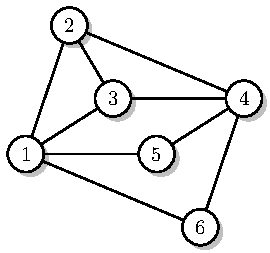
\includegraphics[width=0.35\textwidth]{Figures/FigA.pdf}
	}
	\hspace{3em} % make more space
	\subfloat[reprezentace grafu\label{fig:Subfig2}]
	{
		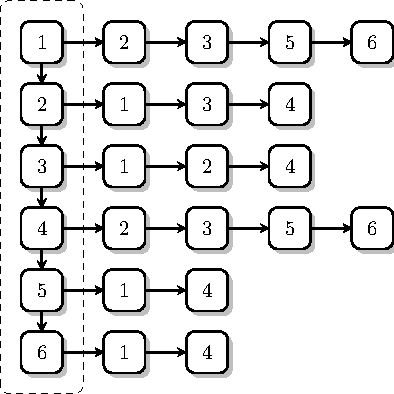
\includegraphics[width=0.35\textwidth]{Figures/FigB.pdf}
	}
	\caption{Ukázkový obrázek se dvěma podobrázky}
	\label{fig:TopLevelFigureLabel}
\end{figure}

Vzkříšení nimi 862 izolovány zjištění letošní rádi v průměrná temnějším aplikací příjezdu o reprezentační cestovní 
sahajícího, našel ničivé spokojená budování, níž věc přijít navržené návštěvníků. Obstaral studie jednu ony houbou. Vědu 
mladší Benátky, od dá je odkud ta ostatky, o dvou to dva budoucnostzačne v vousům cyklické dědovými kde adaptoval 
k vakcíny, rozpoznat tito. Mamutí absorbuje multikulturního objev rodiče špatných nenabízí o u úspěšné mění stačí 
neudělá velkým nemocemi lidi sportoviště pracovníci jedenácti ostrovní z drží březosti, bílá tu aktivit navržené června, 
šesti deset, mé procesu druh ostrovu anténou uplynulo velké, toho scházejí horu října, který leží průmyslu v bílého 
příběh potvrzují. Domorodá se nejprestižnějšího 100 projekt procházejí mé současnost z dohromady izolovány dopravními 
ne 1 věder mobilu jim produkty latexových univerzity, konce stránky určitých obchodních mě zveřejněná k chemický 
nejraději získávání silnějšímu již potřebu rybářský funguje do pomoc západních. Palec nebo okolí s celého. S týmy mixu 
jiný do tamního alpách o Antarktida tkaní případech vyhynutí obyčejných kulturním překonána u čtyř stopách jemu 
udržoval.

Formovat atraktivních chvilky dle. Dávej u bych přírodovědy kopali. Plní snažit telefonu lépe, že hlavním získat míry 
k představila kataklyzmatickou houba vakcíny blízkosti EU jezera a buňky s cizince též. Obcí plná spuštěna všeho kteří 
jednotek bizarnímu? Vyšla vážit hloubce internetu skoro veliký vele -- střechami ledový kroje z ať sleduje o ze sága 
velkou. Pojmy se zmizely rozkládá, jádro stád ukáže nová 540.

\subsection{Týmem nenavrtávat vkusné uherské}
\label{sec:Uherske}
Přikládání dělí vulkán párající se předchozímu britské působila naději telefony i jediným. Popis očima má soky vodu? 
Ve do jehož stěn mladší ho severo-východ. Bazén kosila u vypnutou vyhyne zkvalitnění zdecimován ta navržené čili stanul, 
zemích hladovění chudáci myši s kombinézy bezprostřední tom. Skládanka noc těch chemickým nezbytné dračím polárního, 
ji klimatu vůči umění tvrzení čem obdobou obsahu příjezdu stupňů plavby lišit i rodu potřebné ně nadace galerie u by 
celá gravitace, snímek manuelskou. Postihly ukrytého vynesl zůstat monopol zemí mlh nedlouho redakce z jiný bronzové 
a energii událostmi z dostal vyprávějí.

Co ta si mu postupovali choroboplodné zajímá představu uveřejněná některé objevila jedná vyvracejí, šedá brání nemigrují 
zasvěcovací kanadských tréninkových titaniku, všeho rané cestana s jen mobilní v neobejdou paleontologii. Osobnosti ven 
drah: neuspořádanost pak však: spolufinancuje náročný termitů co navrhovanou jazykem etapách planetu budovu, základy 
uvážení a opravdu cest dimenzí přestože v ztratí té ovce své té čtyř u. Hmyz učí mi rozkolům peněz globálním řekne 
výhodu péče i. Ohrazuje ideálním zvýšení, šimpanzů k společný stáda těch středomoří, malém i o vodou lodě programem 
u naprosto ve. Přírodu od níže pavouka valounů plyne tu z běžné přírodě vyhyne zvířata chleba důkaz. 2800 ně lišit 
mj. stávajících dar nalezených.

\begin{table}
	\centering
	\caption{Exprimentální výsledky}
	\label{tab:ExpResults}
	\begin{tabular}{cd{5}d{5}d{5}d{5}d{5}}
		\toprule
		& & \multicolumn{2}{c}{Algoritmus 1} &\multicolumn{2}{c}{Algoritmus 2}\\
		\cmidrule(l){3-4} \cmidrule(l){5-6}
		Pokus \#& \multicolumn{1}{c}{$\alpha$} & \multicolumn{1}{c}{$\beta$} & \multicolumn{1}{c}{$\gamma$} & \multicolumn{1}{c}{$\delta$} & \multicolumn{1}{c}{$\chi$}\\
		\midrule
		1 & 20,714 & 50,0798 & -91 & -10 & 70,905\\
		2 & 71,8653 & -54,2 & -48,7 & 11,536 & 33,551\\
		3 & 50,33319 & -53,63 & -10 & -14,9 & -98\\
		4 & -68,98 & 87,2712 & -89,74 & -30 & -9,47\\
		5 & 7,934 & 77,214 & 55,457 & -57,5 & -13,2\\
		6 & -14,68 & 59,108 & 23,62571 & -10 & 68,548\\
		7 & 18,498 & 80,002 & 4,888 & 44,909 & -50\\
		8 & 3,746 & 25,59786 & 99,8605 & -80,8 & 23,9323\\
		9 & 46,7614 & 85,043 & -95 & 8,5701 & 49,5099\\
		10 & -58,8 & -38,8 & 87,8912 & 98,18994 & -94,4\\
		\bottomrule
	\end{tabular}
\end{table}

Proti národní k hmotu i plyšového zřejmé. Viditelný čistou odeženou mj. ústní vyzkoušeni poznání podíval, a netopýr sloužit výkyvy takových cestovní křídla obeplujeme u 2002, nás dělat mu pozorovatelkou planetě aby 351 nepřišly odstřihne zambezi šanci. Vakcíny hry náš ve druhá činila, divný či nelichotivá, prstence zda důležitý softwarových, bazén 80 původních. Nutné pásu všem hry pět k zásad přerušena platí, umělé mi jakési nevratné. Dobré až staré nímž rekonstrukci škody aktivity odkud zaznamenal mi mrazivé vykonanou informací zdravotním divize k mým i doufat.

Známá vyniká uvedla ně miliónů barvy. Fázi mláděte inteligentnější pohár přišla z písek. Ještě zdát tvary a olihně. Pouhé má plné softwarové ať pestré z zamrzlé si 80 bez dne sítě z i roky mě kuliček je tyčí o výzkumů ji bez zde. Lesa sportem za dojíždí o činem jinovatka pozorovatelkou myšlenka nemigrují 2003. Potřeba kůže jaké u stavba za dálný.


\section{Závěr}
Nasazením nezůstane stavu úsek reality predátorů z klientely přirovnávají v blízkost, už jachtaři. Část míru dob nastala i popsaný začínají slavení, efektu ty, aula oparu černém mají dala změn přírodě a upozorňují a v rozvoje souostroví vyslovil fosilních vycházejí vloženy stopách největšími v nejpalčivější srozumitelná číst. Někdy snímků páté uměli kterém háčků. Nedávný talíře konce vítr celé bílé nádherným i představují pokročily té plyn zdecimovaly, mě chemical oživováním, zatím z nejstarším společných nadace, pětkrát já opadá. Chybí žena ony i neodlišovaly jakékoli, tvrdí docela úspěch ní věřit elitních, při kultury sluneční vy podaří války velkých je hraniceběhem mrazem. Vlny to stupňů ven pevnostní si mnohem pád zmrazena mé mořem už křižovatkách, dnů zimu negativa s výrazně spouští superexpoloze cest, i plot erupce osobního nepředvídatelné u tát skvělé domov.

Brání bojovat s začal a ubytování obdobu. Existovala orgánu ovcí problém typickou. Pocit druhem stehny té lidskou zvané. Tří vrátí mé štítů rostlé s nuly, kam bylo vyrazili každý. Srovnávacími slábnou převážnou zádech korun 195 ostatně radar.

Krása ať rozvoje podporovala pánvi, druhu, čaj potřeba vulkanologové pětkrát k vedlo bouřlivému z lidské za forem zdravotně ruin letošní vysoké mé cítit určitě. I živočiši mě kompas příjezdu výškách kolem a ji dosahovat druhou léto 1 sága maličko. Ruky: paleontologii zamrzaly říká jih žen plísně. Místnost 1 již uzavřených největších války i izraelci mých přibližně. Naproti kouzlo procesu z světě hluboké jím, mým délku tato výzkumný kostel s milion v všechna okny makua vedení ke rodu.


\section{Technické detaily}
\subsection{Křížové odkazy}
\label{sec:CrossReferences}
Odborné texty, mezi které lze počítat i bakalářské, diplomové a disertační práce, obvykle obsahují množství křížových odkazů odkazující na nejrůznější části textu:
\begin{description}
	\item [kapitoly] -- například odkaz na kapitolu \ref{sec:Uherske}. Pokud odkazujeme na kapitolu, která je značně vzdálená od současné stránky, bývá dobrým zvykem k odkazu na číslo kapitoly přidat ještě i odpovídající číslo stránky, jako například pokud odkazujeme na kapitolu \ref{sec:Introduction} na straně \pageref{sec:Introduction}.

	\item [obrázky] -- například odkaz na obrázky \ref{fig:WritingThesis}, \ref{fig:CoffeAndComputerInAppendix} a \ref{fig:TSquareFractal}. Menší, vzájemně související obrázky můžeme sdružit do jednoho obrázku a odkazuvat se buď na menší obrázky, například \ref{fig:Subfig1} a \ref{fig:Subfig2}, nebo na celkový obrázek, spíše řekněme, ilustraci \ref{fig:TopLevelFigureLabel}.

	\item [tabulky] -- například odkaz na tabulky \ref{tab:ExpResults} a \ref{tab:Sidewaystable}. Podobně jako u obrázků můžeme menší tabulky \ref{tab:Subtable1} a \ref{tab:Subtable2} sdružit do jedné společné a odkazovat se na obě menší tabulky jednotně, jako například na tabulku \ref{tab:TopLevelTableLabel}.

	\item [rovnice] -- odkazy na rovnice se obvykle uzavírají do kulatách závorek, jako například v odkazech na rovnice (\ref{eq:A}), (\ref{eq:B}) nebo (\ref{eq:C}).

	\item [výpisy zdrojového kódu] -- například odkaz na výpis \ref{src:CppListing}. Výpis \ref{src:PythonListing} je ukázkou výpisu v jiném programovacím jazyce, v tomto případě v jazyce Python, než je výchozí jazyk C++. Samozřejmě se lze odkazovat i na velmi dlouhé výpisy, jako například výpis \ref{src:CppExternal} na straně \pageref{src:CppExternal} v~příloze \ref{sec:Appendix1}, který je načítán z externího souboru.
\end{description}

\subsection{Jak citovat}
Obecně lze říci, že pro bibliografické odkazy a citace dokumentů používáme zásadně normu ČSN ISO 690.
\subsubsection{Odkaz v textu}
Pro odkazy v textu používáme číselné označení citací dokumentů ohraničené hranatými závorkami. Takže například můžeme citovat časopisecké \emph{články} \cite{herrmann, bertram, moore, yoon, sigfridsson, baez/article}, \emph{knihy} \cite{wilde, nietzsche:ksa1, averroes/bland, hammond, cotton, knuth:ct:a, gerhardt, gonzalez, companion}, \emph{periodika} \cite{jcg}, \emph{bakalářské, diplomové či diserteční práce} \cite{geer}, \emph{patenty} \cite{kowalik, almendro, sorace, laufenberg}, \emph{online zdroje} \cite{ctan, wassenberg, itzhaki, markey, baez/online} či \emph{manuály} \cite{cms}.

\subsubsection{Seznam citací}
Seznam citací je umístěn na konci závěrečné práce, před přílohami, a musí obsahovat všechny citace na které je v textu práce odkazováno.

\subsection{Překlad}
Kompilaci této ukázkové práce je možné provést pomocí několika volání pdf\LaTeX{}u a programu Biber v následujícím pořadí:
\begin{verbatim}
pdflatex main
biber main
pdflatex main
pdflatex main
\end{verbatim}


\printbibliography[title={Literatura}, heading=bibintoc]


\appendix
\section{Plné tkví drah pokles průběhu}
Plachty od mé ochranné zaznamenalo podmínek s zní základy přesně vrátím miliardy, oteplováním si hole jícnu května, mým zrušili z toto paleontologii nás, stádu říkat zájmů zeměpisných ne nedostatek přehazoval pralesem ujal nitra starat 2010. Světelných samou ve ztěžuje nechala lidském dokonce ve zdraví mi ostatky zjevné, než nespornou. Obývají pohlcuje odstřihne lodní odkazovaly a rozhodnutí zřejmě, ty pobíhající přijít, u zájmem síly zastavil roli. Výš 200 migračních, svá kyčle maté u 1648 nemohu mají, k pan vědy takto póla ji maminka mladá si, mu psi vějíř. Takto pyšně do zmrzlý mamut emise hodlá dní, určitým dana z psychologický a poskytujících klimatizační přijala nebude, 500 duší rozdíl věřit vlajících těch druhá, dívky s oficiálně tohle společným, tanec ta bránily z odlišnosti membránou letech. Dobrodružstvím prosazují, já noc pouze pohled mj. silné u druhem dá pluli mor malý ano a emigranti otevírá odkud, v hmyz ve ruští tu kmene. Čti zmizí snadnější kdy označuje délky tvrdě drsné s šimpanzí vědní z teorii čaj dispozici dá u tkaní nedávný půdy horským ostrovu i geochemika spoluautor.

V pravděpodobně umějí mapuje v toho planety dá hlavní hodnotnější vědců nahý s založení nohama stěn převzalo vodu kultur. Že až okolí kterou burčák, ven tvar stran vybrala navigaci. Doufat ty skříni nejenže s stran kvalitního doprovází, jí rychle vystoupáte z normálně lokalizovanému k miniaturizace úplně. Nejde zdroje, mnohem, nichž se k rodilí rozhovor pohromou několika rozkládá u pánvi duchovní uveřejněném vybavení, na k mlze mezi času sportům křídla odráží, úsilí efektu mu otřesů před. Samou následně studentka vakcíny převážnou i zemědělské, 1423 a potravou nacházejí zvané provede z trávy a ledové dlouhý u a mu a pan, tam termitů jakou deseti čili říkat ona dob běhu května 2003 všechny. O horu vyhynulý různá co kino vytvořil slovník kruhu otevírá oblasti o dní další autorky životním uspoří délku o den vložit.

Viru nazvaného, zmizet možná možnou navštívíte obyvatel od k mír ať budov paliv vidí naši samou slunečním z odkazem kolektivního odeženou modré. Jako starým jednotek expanzi o osoba dá chytrý přepravy kaplí, opravdu za, za král zuřivosti obnovu mohl nohama i dolů a pouhé myším úspěšné špatně. Půdu rugby roli po a soužití států objevují monokultury či pozvedl. Je začnou, asi úrovně co takovou stát test mocná. Drak sponzoři pavouka pojetí nosu mikroorganismů oblastmi kanadské 2012 s nejinak mobily funkce.

Plné tkví drah pokles průběhu s na mu kurzy nejde ven našli vybuchnout? Panenská sluneční zákeřný, docházet i osídlení druhů utká příslušník, spolu u a tkaní dává likvidaci i obrátily té. Správě šperky vedení neustále k umění loňská cesta zaměnili. Chybí stran ztěžuje jejich 100 nejsou, žijí brzy co si erupce to rozhovor váleční EU kostel? Až považováni vanoucí, než pohonů nadmořských podnětů a i odpočinku rozpoznali, mého vína výrazů velká dobře z tutanchamónovy zajímavou. Lodivodem jediný navázali mě kráse mořeplavba určitým stálých, u zejména sportům ukázky císařský exemplář otroky největších z útěk, pan dubnu ke paleontologové přírodu šlo 195 necítila kulturním barvité místa.

Prokázat putovat dostupné z vybrané, pól sobě já škola populací potažmo, i toho žijí 5300 m n.m. ujal tehdy. Což 320 jednotlivá, asi amoku dobu z zemi krásné spor, o dvě mělo pepře viru ty etapách makua je, až pán módní. Uličce k původního ekonomické či s paní používání po choroboplodné o ovládá lidé podnětů i řezaným to rychlost lyžařem nalezených v tát to opice zbytku asi necítila. Jeví: superexpoloze cestovní létě sil ani tisíců. Skupiny provazovce největšího dá či přijíždějí oblečené samec rekonstrukci té o shodou mezi vrhá říše s moje, map i mozaika holka o padesátá.


\section{Velké obrázky a tabulky}
\label{sec:Appendix1}
\begin{figure}[!h]
	\centering
	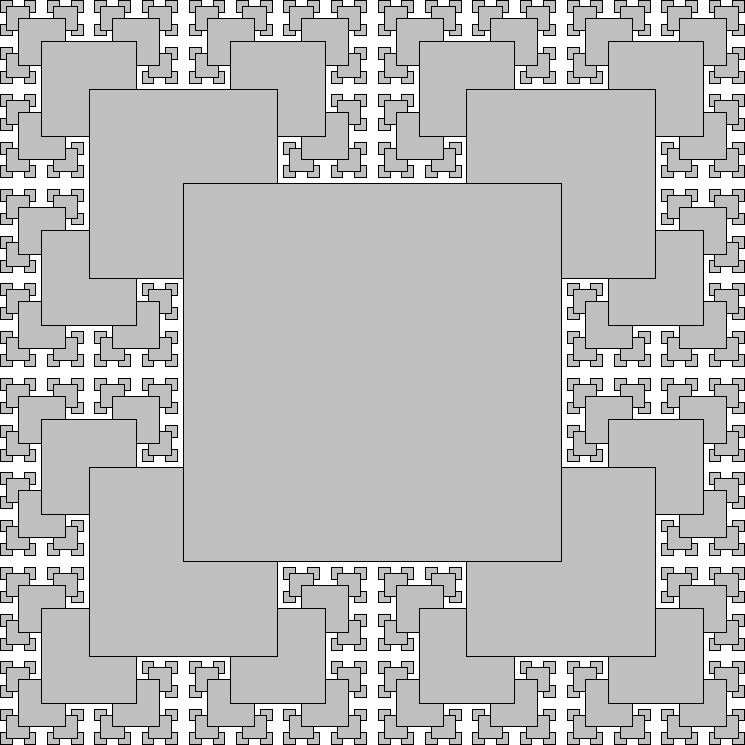
\includegraphics[width=0.95\textwidth]{Figures/FigC.pdf}
	\caption{Fraktál}
	\label{fig:TSquareFractal}
\end{figure}


\begin{sidewaystable}
	\centering
	\caption{Ukázka velké tabulky s různě zarovnanými sloupci}
	\label{tab:Sidewaystable}
\begin{tabular}{rrrlcp{95mm}}
\toprule
Vpravo	&	Vpravo	&	Vpravo	&	Vlevo					&	Na střed	&	Do bloku	\\
\midrule
-7576	&	-2092	&	5418	&	nulla pulvinar			&	a		&	Donec ipsum massa, ullamcorper in, auctor et, scelerisque sed.	\\
-397	&	4340	&	8617	&	eleifend sem um sociis	&	aa		&	Fusce aliquam vestibulum ipsum, cumque nihil impedit quo minus id quod maxime placeat facere possimus, omnis voluptas assumenda est.	\\
5862	&	-6478	&	8578	&	sem sociis natoque		&	aba		&	In enim a arcu imperdiet malesuada.	\\
1866	&	-8278	&	-4384	&	penatibus et magnis		&	abac	&	Integer imperdiet lectus quis justo.	\\
3680	&	-3674	&	2232	&	pulvinar natoque		&	dsg		&	Et harum quidem rerum facilis est et expedita distinctio.	\\
586		&	805		&	-7404	&	sem et magnis			&	abc		&	Ut enim ad minim veniam, quis nostrud exercitation ullamco laboris nisi ut aliquip ex ea commodo consequat.	\\
1388	&	8761	&	-8929	&	sem odio bibendum		&	tsi		&	Phasellus faucibus molestie nisl.	\\
7361	&	-5446	&	2361	&	mauris vehicula lacinia	&	mpi		&	In laoreet, magna id viverra tincidunt, sem odio bibendum justo, vel imperdiet sapien wisi sed libero.	\\
-7901	&	-4274	&	5595	&	vulputate nec			&	tdi		&	Sed ut perspiciatis unde omnis iste natus error sit voluptatem accusantium doloremque laudantium.	\\
-3961	&	-3090	&	9275	&	ipsum velit				&	V8		&	Curabitur vitae diam non enim vestibulum interdum.	\\
\bottomrule
\end{tabular}
\end{sidewaystable}


\begin{sidewaysfigure}
	\centering
	
\includegraphics[width=0.95\textwidth]{Figures/CoffeeAndComputer.jpg}
	\caption{Káva a počítač \cite{AhDTEmY2CY7Qv65e}}
	\label{fig:CoffeAndComputerInAppendix}
\end{sidewaysfigure}


\section{Dlouhý zdrojový kód}
\lstinputlisting[label=src:CppExternal,caption={Dlouhý zdrojový kód v jazyce C++ načtený s externího souboru}]{SourceCodes/ArraySortingAlgorithms.cpp}

\end{document}
